\documentclass[12pt,draft]{mitthesis} 

\usepackage{lgrind, braket, amsmath,
  amssymb, bbm, booktabs, subfig, color} 

\usepackage[pdftex]{graphicx}
\usepackage[version=3]{mhchem}

\newcommand{\TODO} [1]{\textcolor{magenta}{\textbf{TODO:} #1}}
\newcommand{\NOTE} [1]{\textcolor{magenta}{[\emph{#1}]}}
\newcommand{\POINT}[1]{\textcolor{magenta}{#1}}

\newcommand{\rcm}{cm$^{-1}$}
\newcommand{\bigspace}{$
  \;
  $}

\newcommand{\astate}{$
  \tilde{\text{A}} \: ^1\!A_u
  $}
\newcommand{\AtoX}{$
  \tilde{\text{A}} \: ^1\!A_u 
  \leftarrow 
  \tilde{\text{X}} \: ^1\Sigma_g^+
  $}
\newcommand{\StoS}{$
  S_1 \leftarrow S_0
  $}
\newcommand{\microsec}{$\mu$s}

\hyphenation{acetylene}
\hyphenation{Hamiltonian}

\begin{document}

\tableofcontents
\clearpage

\subsubsection*{NOTES}

\clearpage

\setcounter{chapter}{4}
\chapter{Contrasting singlet$\sim$triplet dynamical behavior of two
  vibrational levels of the acetylene $S_1$ $2^13^1B^2$ polyad }

\section{Introduction}


% \POINT{Make the case for studying non-symmetric bending motions in
%   acetylene.  The $T_3$ state is bent out-of-plane.  However, several
%   observations have been made that mode 6 is more active in promoting
%   ISC.  How does this jive with our distant doorway theory?}
\TODO{Adapt from article}.  The $\tilde{A} ^1A_u \leftarrow \tilde{X}
^1\Sigma_g^+$ electronic band system of acetylene is one of the most
thoroughly examined electronic transitions of any polyatomic molecule.
Several researchers have used double resonance techniques to detect
and analyze transitions to the $\nu_4$ and $\nu_6$ fundamentals,
overtones, and combination bands in the Ã1Au state. Utz et. al. were
the first to unambiguously assign electronic transitions to the
$\tilde{A}$ $^1A_u$ state $\nu_4$ (torsion) and $\nu_6$ (antisymmetric
in-plane bend) vibrational fundamentals using pulsed laser double
resonance in a room temperature cell \cite{utz93}.  They observed
strong $a$- and $b$-axis Coriolis interactions between the two nearly
degenerate bending modes, and deperturbed these interactions to obtain
vibrational frequencies, Coriolis interaction constants, and
rotational constants.  That experiment is very relevant to the work
presented in this paper, since the near degeneracy of the two
vibrational fundamentals is expected to result in analogous
interactions amongst the higher lying combination and overtone levels
involving $\nu_4$ and $\nu_6$.21 Mizoguchi et. al. also observed
ungerade vibrational states via the \AtoX\ transition using IR-UV
double resonance spectroscopy.22 In particular, they excited acetylene
to its ungerade n$\nu$3' + $\nu_4$' and n$\nu$3' + $\nu_6$' (n = 2,3)
vibrational levels in the Ã1Au state via IR excitation of selected
rotational levels in the $\nu$3” vibrational state of the X 1Σg+
electronic ground state.  They investigated the Coriolis coupling
between the combination bands involving $\nu_4$' and $\nu_6$', and
examined the vibrational mode dependence of the singlet $\sim$ triplet
interaction by observing splittings in the $K_a$ = 1 rotational levels
of the 3$\nu$3' + $\nu_6$' band. The singlet $\sim$ triplet
interaction in these states was further probed in continuing work by
Yamakita and Tsuchiya,23 who observed Zeeman quantum beats by IR-UV
double resonance LIF. They observed both rotational level splittings
and Zeeman quantum beats in the fluorescence decay of the $3\nu_3' +
\nu_6'$ band.  No analogous splitting or Zeeman quantum beats were
seen in the $3\nu_3' + \nu_4'$ band. They concluded that excitation of
the out-of-plane $\nu_4$' torsional mode suppresses the singlet $\sim$
triplet interaction, while excitation of the in-plane antisymmetric
bend, $\nu_6$', promotes $S_1$ $\sim$ $T_3$ interaction. From this, it
was inferred that the singlet $\sim$ triplet mixing occurs in a planar
(C2h or C2v) geometry rather than at a non- planar C2 geometry, since
the 3$\nu$3' + $\nu_4$' band did not exhibit any rotational line
splittings or Zeeman quantum beats.  \TODO{Adapt material from
  president's report.}

\POINT{Recent breakthrough in our understanding of these bending
  polyads.  Energies and eigenvectors predicted by AHS and Merer.  The
  out-of-plane bending mode in acetylene $S_1$ is strongly mixed with
  the antisymmetric in-plane bend, so we must study them in tandem.}
\TODO{Adapt from paper.}  Despite numerous investigations, only a
partial picture of $\tilde{A} ^1A_u$ state vibrational structure and
interactions has been developed.  In the normal mode model of
acetylene vibrational dynamics, $\nu_4$ is the only normal vibration
in the Ã1Au state that involves a motion out-of-the-plane from the
planar, trans-bent equilibrium structure of the à state, while $\nu_6$ is
an in-plane antisymmetric bend. A more sophisticated polyad model24
goes beyond the zero-order normal mode picture by incorporating
anharmonic and vibration-rotation (including Coriolis) interactions
among groups of near degenerate states. The results of such an
analysis show that the resultant eigenstates formed from the
zero-order degenerate bending modes are profoundly mixed via strong
anharmonic (Darling-Dennison) and Coriolis interactions.25 In this
case, the simpler normal mode model is invalid, and the vibrational
wavefunctions of levels assigned to $\nu_4$ or $\nu_6$ do not resemble the
nuclear motions suggested by their labels, but are strongly mixed
superpositions of the two zero-order bending modes.  In this work, the
nominal $4^2$ and 62 spectral labels are retained, despite the fact
that the two levels are nearly 50:50 mixed.

\POINT{Section 3 summary.}  The focus of the next section is a
comparison of combination bands involving overtones of the low-
frequency bending vibrations, $\nu_4$ and $\nu_6$, of acetylene in its
$\tilde{A} ^1A_u$ state.

\TODO{Adapt from paper.}  We report on the simultaneously recorded
SEELEM and LIF spectra that sample the near- degenerate, strongly
mixed $2^13^14^2$ $K_a$ = 1 and 213162 Ka = 1 vibrational levels of
acetylene in its Ã1Au state. The SEELEM spectra of these two
vibrational levels are remarkably different. The spectra provide a
unique opportunity to investigate the effect of selective vibrational
excitation on the interaction between singlet and triplet states of
acetylene. One might expect the intensities in the SEELEM spectra of
the $2^13^14^2$ and $2^13^16^2$ vibrational levels to be controlled by
Franck-Condon overlap between the vibrational wavefunctions of the
interacting $S_1$ and $T_3$ electronic states. The expectation under a
normal mode model is that, since the $T_3$ electronic state has a
non-planar Cs configuration,26,27 excitation of the in-plane $\nu_6$ mode
would result in small vibrational overlap with T3, while excitation of
the out-of-plane vibration, $\nu_4$, would result in large vibrational
overlap. If the normal mode model were valid, interaction with triplet
states would be promoted by excitation of $\nu_4$, resulting in large
SEELEM signal, while excitation of $\nu_6$ should suppress SEELEM
activity. The strongly mixed nature of the Ã1Au 213142 $K_a$ = 1 and
$2^13^16^2$ $K_a$ = 1 vibrational levels rules out such a simple
explanation for the contrasting SEELEM spectra observed in the
experiment. The purpose of this paper is to provide an explanation of
the difference between the SEELEM spectra involving the mixed 213142
and $2^13^16^2$ vibrational levels, and to propose a qualitative
mechanism which gives rise to the different spectral
patterns. Comparison and analysis of the SEELEM / LIF spectra will
elucidate the mechanism of the doorway S1$\sim$T3 interaction process.

\section{Experiment}

\TODO{Adapt from previous chapter.}

\section{Results}

\TODO{Make survey figure showing the energy of all investigated bands,
  overlayed on acetylene LIF spectrum.}


\TODO{Adapt the following from the paper.}

Figure \ref{fig:spectrum-2131b2}(a) shows the SEELEM (plotted upward)
and LIF (plotted downward) spectra for the $\tilde{A}^1A_u \leftarrow
\tilde{X}^1\Sigma_g$ nominal $2^13^14^2$ $K_a$=1 $\leftarrow$ $0_0$ Q
and R branch rovibronic transitions of acetylene near 46195 cm-1. The
SEELEM and LIF spectra are very similar for this band in terms of both
frequencies and relative intensities, with the exception of the
anomalously weak LIF Q(1) feature. Each SEELEM feature in the spectrum
is localized in energy near an LIF partner feature. No splitting of
the rotational lines in the LIF spectrum is observed at the 0.06 cm-1
resolution.

Figure \ref{fig:spectrum-2131b2}(b) presents the SEELEM / LIF spectra
for the $\tilde{A}^1A_u \leftarrow \tilde{X}^1\Sigma_g$ nominal
$2^13^16^2$ $K_a$=1 $\leftarrow$ $0_0$ P, Q and R branch transitions
near 46090 cm-1. The SEELEM spectrum of $2^13^16^2$ is remarkably different
from that of 213142. The overall SEELEM signal in $2^13^16^2$ is weaker
than that of $2^13^14^2$ by nearly a factor of 3, even though the LIF
intensity in $2^13^16^2$ is a factor of 3 stronger than that of 213142.  In
213162, the SEELEM features are not well correlated in intensity with
the corresponding features in LIF. In fact, in several cases where a
strong LIF feature appears, the partner SEELEM feature is near or
completely below the noise level. The observed pattern of SEELEM
features in $2^13^16^2$ suggests a significant J' dependence to the SEELEM
activity, and hence, to the interaction of the bright singlet state,
S1, with the perturbing triplet state, T3.

\begin{figure}
  \caption{
    % Simultaneously recorded LIF and SEELEM spectra of the
    % acetylene $2^1_0V^1_04^2_0K^1_0$ and $2^1_0V^1_04^2_0K^1_0$
    % $\tilde{A}^1A_u \leftarrow \tilde{X}^1\Sigma_g$ transitions.  
    % Ripped off from paper.
    (a) Simultaneously recorded surface electron ejection by laser 
    excited metastables (SEELEM, upper trace) and ultraviolet 
    laser-induced fluorescence (UV-LIF, lower trace) spectra of the 
    $2^13^14^2$ $K_a$=1 sublevel of the $\tilde{A}^1A_u \leftarrow
    \tilde{X} ^1\Sigma_g^+$ electronic transition.  (b) P, Q, and R
    branch features of the SEELEM and LIF spectra of the $2^13^16^2$ 
    $K_a$=1 sublevel. The weak Q branch features, which are overlapped 
    with the R branch features of $2^13^16^2$ $K_a$=1, belong to a 
    sublevel of a different polyad.
  }
  \label{fig:spectrum-2131b2}
  \centering
  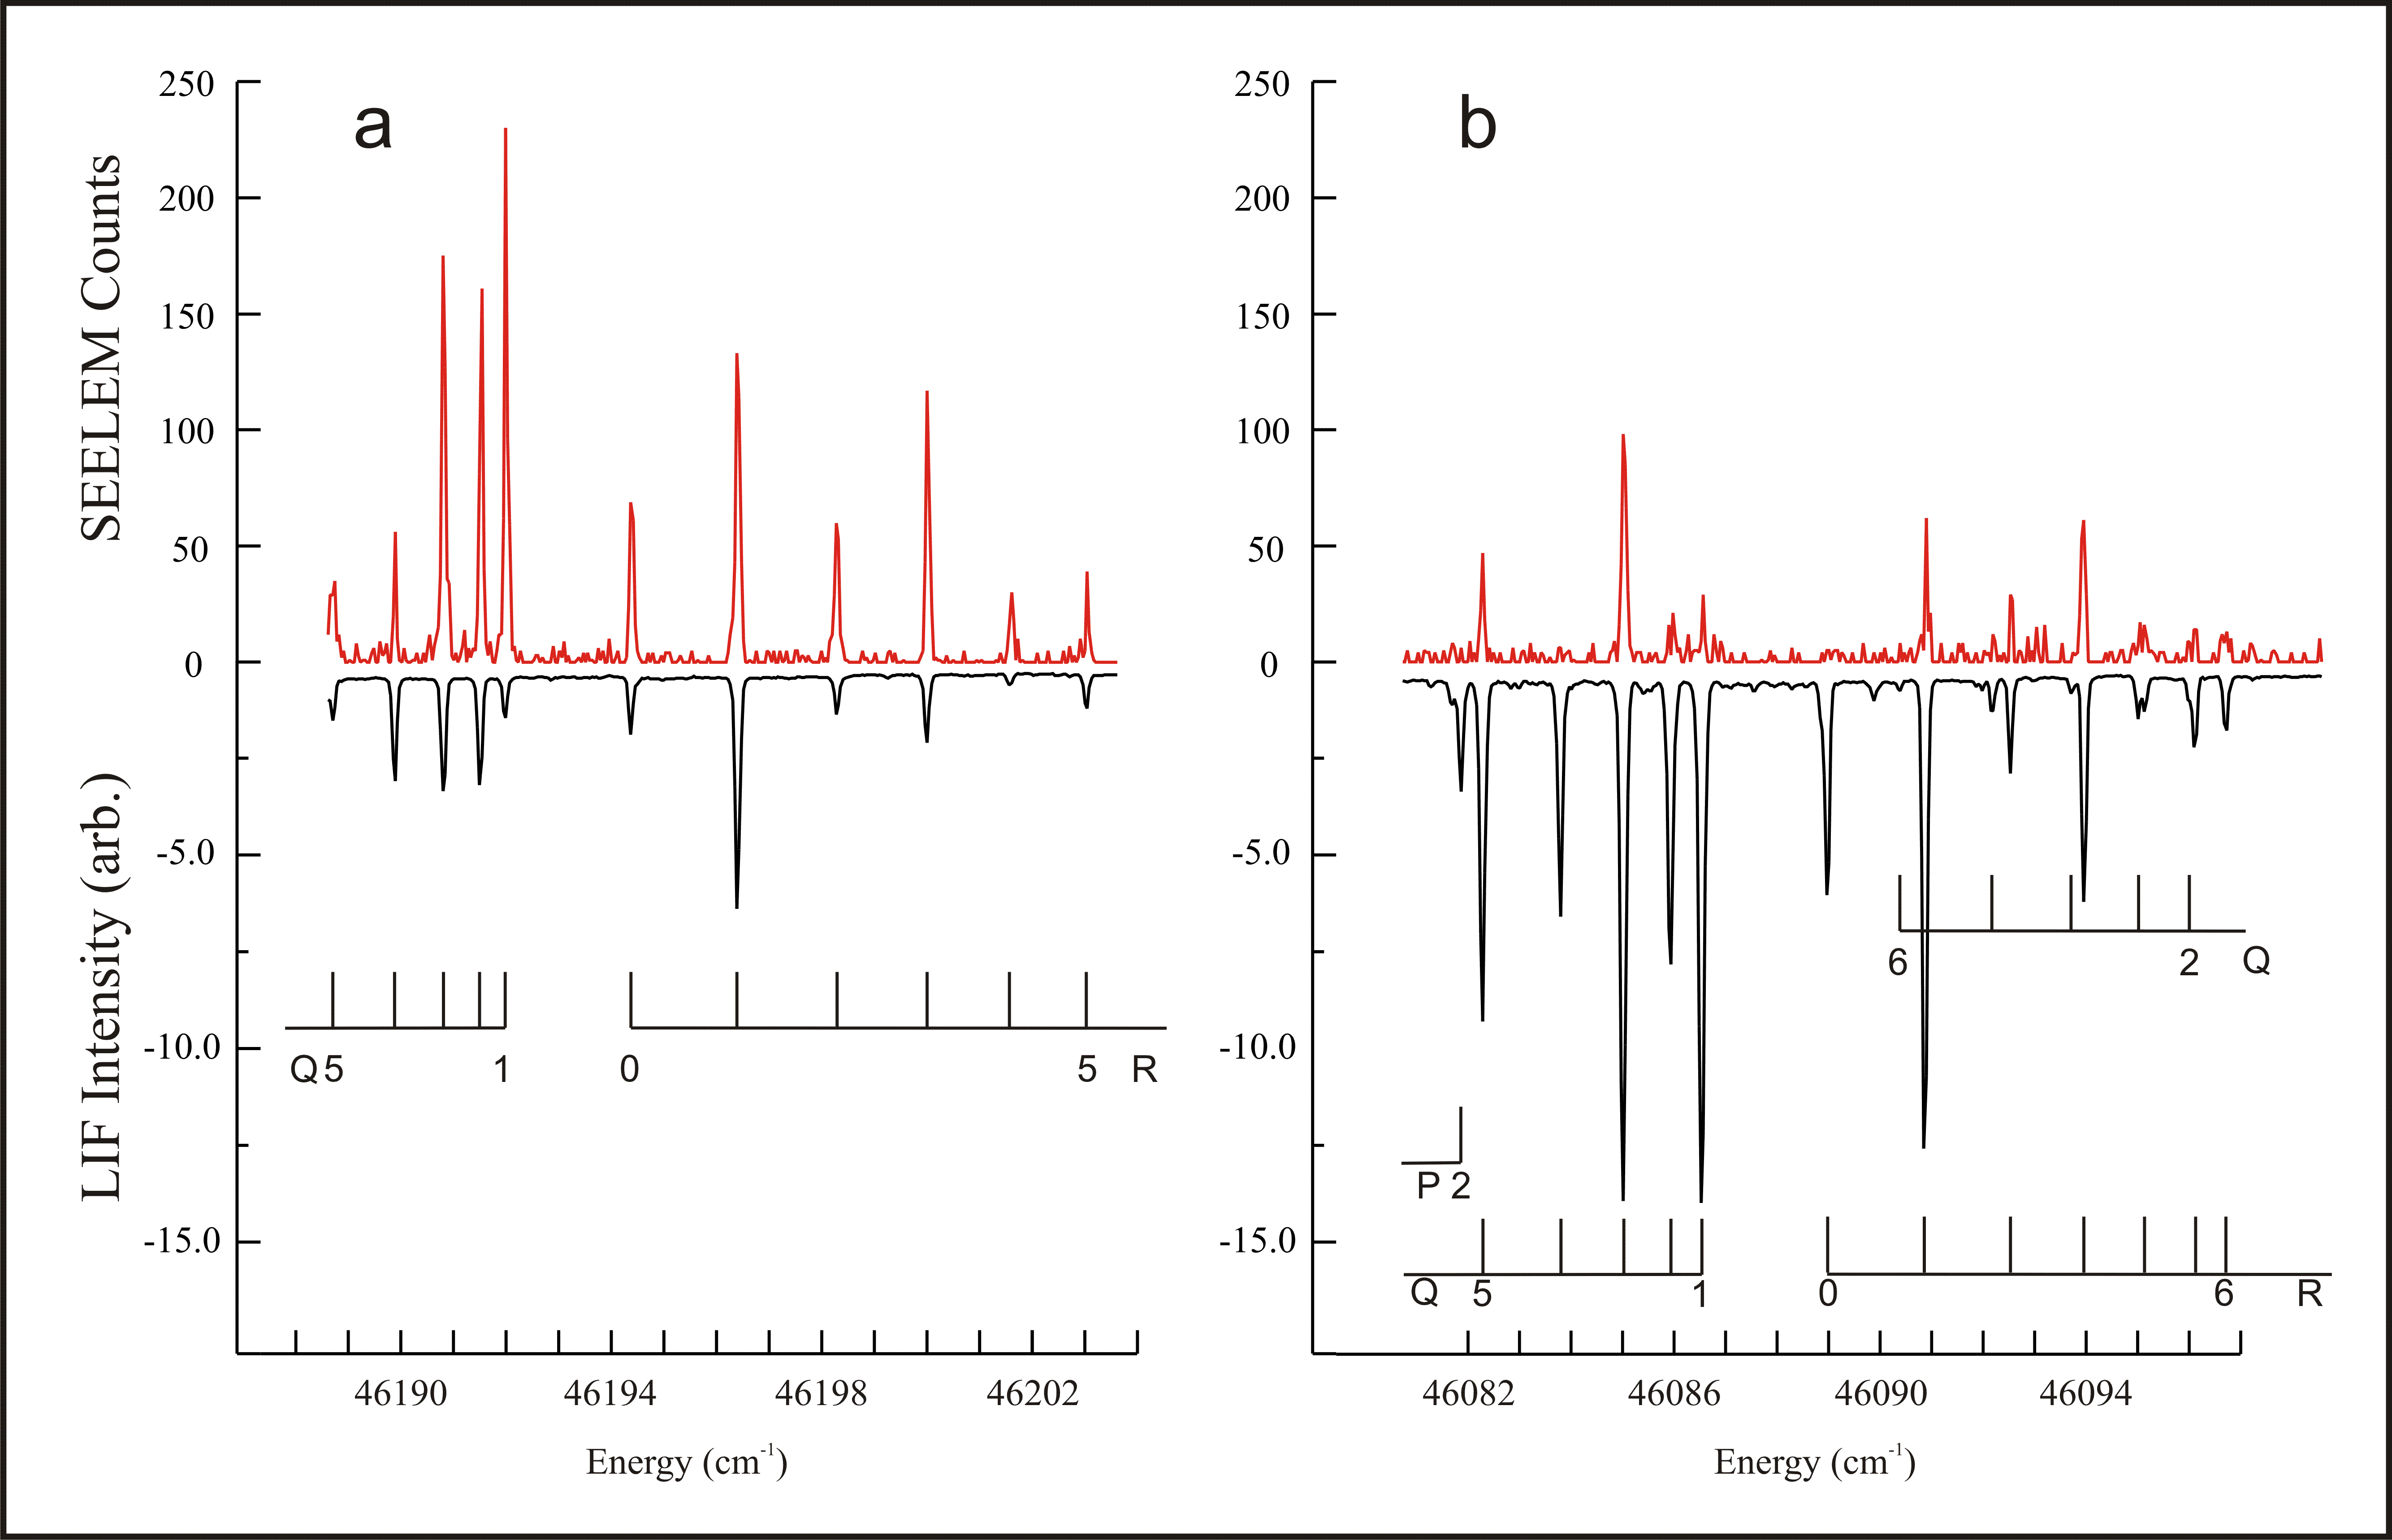
\includegraphics[width=7.5in,angle=90]{spectrum-2131b2.png}
\end{figure}

\section{Analysis: LIF/SEELEM intensity distributions}

\POINT{Results of 2131b2 spectra c.o.g. analysis.}

\POINT{Make the case for center of gravity metric. Use tools from
  Chapter 2.  Summarize and refute arguments against.  (See p.109 of
  4/2007--8/2007 notebook.)}

\POINT{Use gated fluorescence and SEELEM intensity comparison to make
  the case for weak coupling. Lifetimes tabulated in notebook
  8/2007--10/2007.  Weak/strong coupling in c.o.g. analysis is
  counter-intuitive.}

% \POINT{Lifetimes do not match intensities -- does this point to
%   complicated coupling?  (See p.99 of 8/2007--10/2007 notebook, and
%   p.31 of 4/2007--8/2007 notebook.)}

\section{Analysis: Unexpected band intensities resulting from
  competing Coriolis and Darling-Dennison interactions}

\TODO{Adapt analysis from paper.}  While spectra involving vibrational
excitation have been traditionally analyzed in terms of normal modes,
it is well known that at significant excitation energy, the modes can
become strongly mixed, and large deviations from the small-amplitude,
rigid-molecule normal vibrations are expected.  In the case of the
$\nu_4$ and $\nu_6$ bending vibrations of $\tilde{A}$-state acetylene,
the pure normal mode description is not adequate. Superpositions of
normal modes are required to describe the wavefunctions of levels
involving the low-frequency excited state bending vibrations.

Though no deperturbation of the $2^13^1B^2$ polyad has been attempted,
the qualitative structure of the polyad can be anticipated by drawing
parallels to the $B^2$ polyad, which has recently been analyzed by
Merer et al.  In that work, an effective, multiresonant Hamiltonian
was constructed to take into account the effects of Darling-Dennison
resonance in addition to the $a$- and $b$-axis Coriolis interactions
described by Utz and coworkers.  This effective Hamiltonian was fitted
to the available experimental data from the high-sensitivity LIF
spectra of the $B^2$ polyad (containing the $4^2$ ($a_g$), $6^2$
($a_g$), and $4^16^1$ ($b_g$) basis states) recorded in a molecular
beam. It was found that the strength of the Darling-Dennison
interaction is sufficient to cause nearly complete ($\sim$50:50)
mixing of the $4^2$ and $6^2$ basis states in the $J$=$K_a$=0
levels. In the absence of other effects, the nominal $4^2$ and $6^2$
levels would contain the same fractional contributions from the $4^2$
and $6^2$ basis states and would only differ in the phase of that
mixing.  The $4^16^1$ state remains essentially pure in $J$=$K_a$=0.

For levels with $J>0$, the Coriolis interactions must be
considered. In particular, we focus on the $K_a$=1 sublevels that, as
a consequence of the c-type selection rules for the $\tilde{A}^1A_u
\leftarrow \tilde{X} ^1\Sigma_g^+$ transition, dominate the LIF
spectrum recorded from the ground ($\ell"$=0) vibrational level. In
$K_a$=1, the 2:2 Darling-Dennison interaction strongly mixes the
near-resonant $4^2$ and $6^2$ zero-order levels, as it does in
$K_a$=0. However, in $K_a$=1, the a-axis Coriolis matrix elements now
connecting the $4^16^1$ state to the $4^2$ and $6^2$ basis states have
opposite phases. If the Darling-Dennison interaction is
prediagonalized, the phases of the Coriolis matrix elements result in
a strong interference effect. The nominal $4^2$ level has the proper
phase to mix strongly with the $4^16^1$, $b_g$ vibrational symmetry
level, whereas the nominal $6^2$ level has the wrong phase.

Extending this argument to the $2^13^1B^2$ polyad, the strongly mixed
nature of $2^13^14^2$ and $2^13^16^2$ permits $2^13^14^16^1$ to
interact with only one of the two mixed vibrational levels. An
analysis of this interference effect, which depends on the relative
phase of the anharmonic and Coriolis matrix elements, shows that the
 $2^13^14^16^1$ basis state is strongly Coriolis coupled to the nominal
$2^13^14^2$ level but not to the nominal $2^13^16^2$ level. As a result
of the interference effect, a significant amount of $b_g$ character is
mixed exclusively into $2^13^14^2$.

Although this preliminary, semi-quantitative analysis is based on a
local fit of the interactions within $B^2$, rather than a more global
model for all of the $S_1$ bending polyads of acetylene, the interactions
most pertinent to the observed SEELEM spectra can be characterized
using this simple, local model.

\POINT{Contrasting behavior of modes 4 and 6 attributed to differing
  amounts of $b_g$ vibrational character -- they are otherwise
  completely mixed.}

\POINT{Could the amount of $b_g$ character be J-dependent?}

\section{Discussion}

\TODO{Adapt from paper.}  Even a qualitative analysis of the SEELEM
spectra can reveal salient features of the singlet $\sim$ triplet
interaction dynamics. Despite the fact that the LIF signal in
$2^13^16^2$ is a factor of 3 larger than the LIF signal of
$2^13^14^2$, the corresponding SEELEM spectra do not share this same
intensity ratio. In stark contrast to the LIF signal, the SEELEM
signal for $2^13^16^2$ is exceedingly weak, while the $2^13^14^2$
SEELEM signal is comparatively intense. This difference in SEELEM
activity can be interpreted in terms of the strength of the
interaction between the bright $S_1$ state and a unique perturbing
vibrational level of $T_3$.

It is known that the singlet $\sim$ triplet interaction mechanism in
the $\tilde{A}^1A_u$ state of acetylene is a doorway-mediated process,
where the coupling of $S_1$ to the dark $T_{1,2}$ states is mediated
by $T_3$.  In light of the doorway model, there are two possible
explanations for the difference between the two SEELEM spectra. The
first is a vibrational overlap argument, where vibrational overlap
between the $S_1$ and $T_3$ vibrational wavefunctions promotes or
suppresses SEELEM signal. A second possibility is that the phases of
the $a$-axis Coriolis matrix elements connecting the $4^16^1$ state to
the $4^2$ and $6^2$ basis states result in an interference effect that
gives rise to a difference in how the two $S_1$ vibrational levels
interact with $T_3$.

In the normal mode model, $\nu_4$ and $\nu_6$ normal vibrations are
rigorously conserved. In a more accurate polyad model, $2^13^16^2$ and
$2^13^14^2$ belong to a strongly mixed superposition of modes, rather
than pure normal modes. Since the vibrational levels are strongly
mixed, a simple Franck-Condon argument would predict the SEELEM
spectra of $2^13^16^2$ and $2^13^14^2$ to be nearly identical.

The simplest explanation for the difference between the two observed
SEELEM spectra lies in an investigation of the Coriolis interaction
within the mixed $2^13^1B^2$ $K_a$=1 polyad. From the effective
Hamiltonian analysis, the main difference between the wavefunctions of
the two $S_1$ $2^13^1B^2$ vibrational levels probed in the experiment
is the amount of admixed $b_g$ vibrational character, taking into account
the interference between anharmonic and Coriolis interaction matrix
elements. Although $2^13^14^16^1$ is both short-lived and would
fluoresce strongly, it is not easily visible in either SEELEM or LIF
spectra due to low excitation probability and spectral overlap with
the near degenerate $1^13^1$ $K_a$=1 level. Since the a-type Coriolis
interaction causes $2^13^14^16^1$ to interact with (nominal)
$2^13^14^2$, but not with (nominal) $2^13^16^2$, a logical conclusion
is that the $b_g$ vibrational character in the nominal $2^13^14^2$ level
is what gives rise to the enhancement in SEELEM intensity. The
interaction of nominal $2^13^14^2$ with $T_3$ is due to the mixing of
$b_g$ vibrational character into nominal $2^13^14^2$.

While $a$-type Coriolis coupling gives rise to the SEELEM signal in the
region of $2^13^14^2$ $K_a$=1, $b$-type Coriolis coupling may
contribute to the $J$-dependence of the SEELEM signal near the LIF
spectrum of $2^13^16^2$ Ka=1.  The scaling of the $b$-axis Coriolis
matrix elements goes as $\sqrt{J(J+1)-K(K+1)}$ , which results in strongly
$J$-dependent mixing between basis states differing in both $K_a$ and
the vibrational quantum numbers. This strong $J$-dependence also leads
to states with anomalous effective rotational structure. Since the
higher $K_a$ sublevels of $2^13^14^16^1$ can mix with the nominal
$2^13^16^2$ $K_a$=1 level, these are likely candidates for the sources
of $b_g$ character, which is shown here to be essential to the
interaction with the nearby $T_3$ level.

% \section{Investigation of ``pure bending'' vibrational levels:
%   $4^16^3$ and $4^3$}

% \subsection{Results}

% \TODO{Figures of spectra for these bands (with assignments)}

% \POINT{SEELEM spectrum of $4^1 6^3$ is very weak (See data from Feb 2,
%   p.50 of 1/2007--3/2007 notebook.)}

% \POINT{SEELEM spectrum of $4^3$ $K=2$ hot band (Jan 16A) -- need to
%   check this in Watson's atlas.}

% \subsection{Analysis and discussion}

% \POINT{Discuss in terms of global structure of bending polyads.  (See
%   AHS and Merer's predictions on p.39 of 1/2007--3/2007 notebook.)}

% \POINT{The conclusion is that we probably don't have enough S/N with
%   these bands to perform any SEELEM/LIF intensity analysis.  Can we
%   get any amount of info from lifetimes or quantum beats?}

% \POINT{Uniformity of coupling in both Q and (P,R) branches -- does
%   this imply that $K\ne0$?}

\section{Conclusion}

\TODO{Adapt from paper.}  SEELEM / LIF spectra of two related bands in
the $\tilde{A}^1A_u \leftarrow \tilde{X} ^1\Sigma_g^+$ system of
acetylene have been recorded in order to elucidate the nature of
S1$\sim$T3 interaction in acetylene. A simple model is proposed which
explains the intensity effects and features in the contrasting SEELEM
spectra in the region of the $2^13^16^2$ and $2^13^14^2$ vibrational
levels. The $2^13^16^2$ $K_a$=1 and $2^13^14^2$ $K_a$=1 vibrational
levels are strongly mixed by anharmonic Darling-Dennison
interactions. The major difference between these two $S_1$ vibrational
levels is the significant amount of $b_g$ vibrational character mixed
into $2^13^14^2$ by a-axis Coriolis coupling. This gives rise to
enhanced S1$\sim$T3 mixing in the nominal 213142 level, as observed.
When examined together, both the SEELEM / LIF experiment and polyad
theoretical arguments add important new details about the nature of
the doorway mediated mechanism for intersystem crossing in acetylene.

\POINT{Darling-Dennison and A-type Coriolis coupling play a major role
  in determining the singlet-triplet interactions for vibrational
  levels involving modes 4 and 6.}

\POINT{Make the case for studying the bending motions without
  complications from Darling-Dennison or $a$-type Coriolis coupling.}



\bibliography{master}
\bibliographystyle{plain}
\end{document}
